\begin{figure}[t]
	\begin{center}
		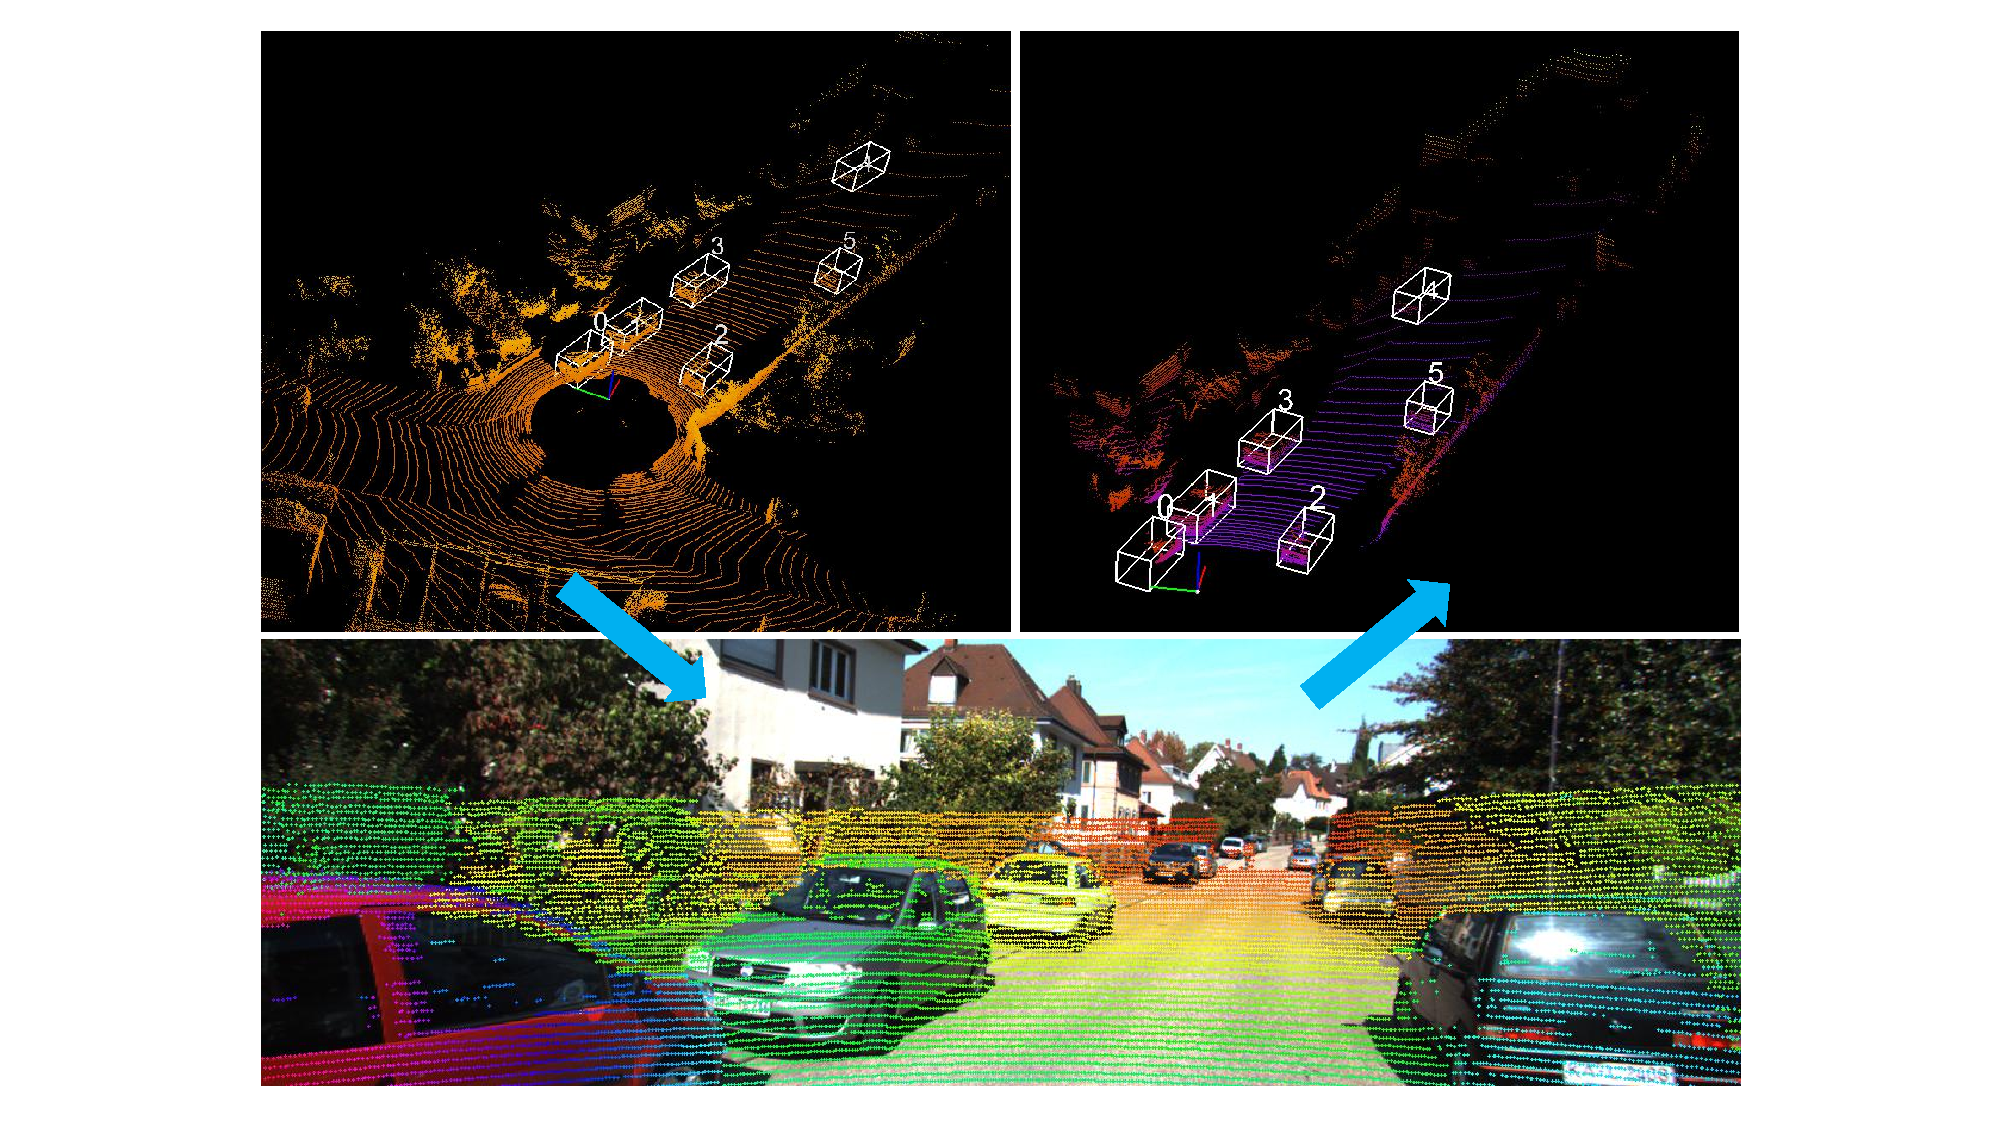
\includegraphics[trim={5cm, 0.5cm, 5cm, 0.5cm}, clip, width=\textwidth]{imgs/projection.pdf}
	\end{center}
	\vspace{-0.8cm}
	\caption{将三维点云数据投影到图像平面,然后保留落在图像边界内的点云,使点云数据与图像数据范围保持一致,有利于数据融合。}
	\label{fig:projection}
	%\vspace{-0.3cm}
\end{figure}
